\documentclass{article}
\usepackage[utf8]{inputenc}
\usepackage[spanish]{babel}
\usepackage{graphicx}
\usepackage{amsmath}
\title{Modelos Matemáticos Discretos}
\author{Juan Diego Omaña Avila}
\begin{document}
\maketitle
\section{Ecuaciones en diferiencias.}
\subsection{Primer orden}
Sabemos que $$\lim_{x\to\infty}\frac{1}{x}=0$$

Para encontrar este resultado ocupamos que $$\sum_{i=0}^{n-1}a^i=\frac{1-a^{n}}{1-a}$$

La ecuacion $x_{n+1}=ax_n+b$ se llama una ecuacion en diferiencia de primer orden linealcon coeficientes constantes no Homageneos.

Algunos valores de la invercion:
\begin{center}
\begin{tabular}{|c|r|}
\hline
Mes & Valor\\
\hline
0 & 1000 \\
1 & 1010 \\
2 & 1021.10 \\
3 & 1030.301 \\
\hline
\end{tabular}
\end{center}

Una gráfica del resultado es:

\begin{center}
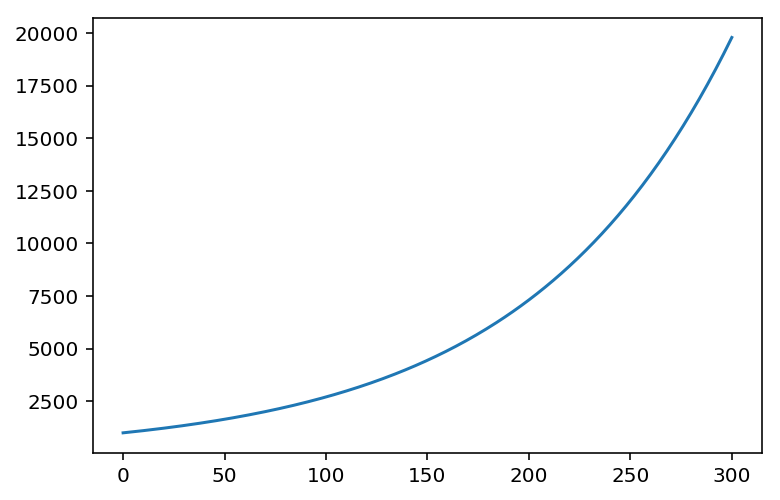
\includegraphics[width=8cm]{GRAFICA}
\end{center}

Tenemos \$1000 que vamos a invertir a un interes del 1\% mensual.

El valor de la invercion cuando han trascurido $n$ meses es $$x_n=1000(1.01)^n$$.
\subsection{Segundo orden}
\end{document}
